\chapter{Estado del arte}\label{cap.estado}
Una vez descrito el contexto general de este TFM, en este capítulo se profundiza en redes neuronales para detección visual de objetos en imágenes, puesto que serán la base principal del procesamiento visual necesario en el comportamiento sigue-persona. Estas redes neuronales se entrenan típicamente con grandes bases de datos con objetos etiquetados. Se presentan en este capítulo las más relevantes.
\section{Redes neuronales para detección visual de objetos}
\label{sec:nets}

Rigoberto Vizcay~\cite{tesis_rigoberto} se basa en redes \textit{\acrfull{cnn}} para la detección de vehículos y peatones. Una red neuronal convolucional es una red que presenta una o varias capas convolucionales. La red que implementó constaba de dos capas de convolución y dos de agrupamiento, además de la capa de salida completamente conectada. En la Figura~\ref{fig.cnn_estado_arte} se puede ver la estructura de la red.

\begin{figure}[H]
  \begin{center}
    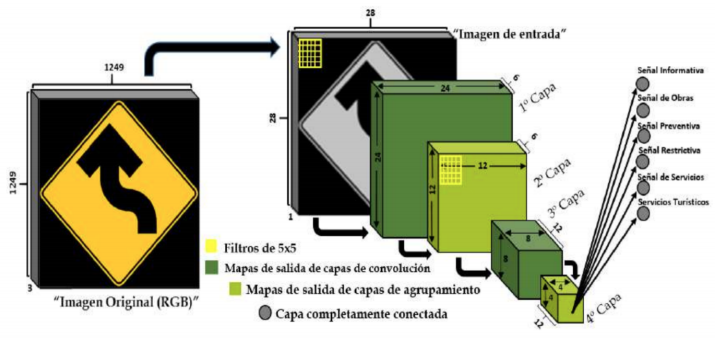
\includegraphics[width=0.7\textwidth]{figures/estado_arte/cnn.png}
		\caption{CNN Rigoberto Vizcay~\cite{tesis_rigoberto}}
		\label{fig.cnn_estado_arte}
		\end{center}
\end{figure}

Y. Abdullah, G. Mehmet, A. Iman and B. Erkan~\cite{rcnn_detection}  plantean el uso de \textit{\acrfull{rcnn}} y Faster \acrshort{rcnn} para la detección de vehículos. Por un lado, \acrshort{rcnn} para realizar las detecciones realiza tres fases que se pueden ver en la Figura~\ref{fig.rcnn}:
\begin{enumerate}
    \item Se emplea el algoritmo \textit{Selective Search}, el cual solo realiza las pruebas de detección a las regiones candidatas a tener una posible detección. Con ello se extraen aproximadamente 2000 regiones de la imagen (\textit{Region Proposal}).
    \item Se implementa una red neuronal \textit{\acrfull{cnn}} en la parte superior de cada región.
    \item Se extrapola la salida de cada \acrshort{cnn} y se ingresa en una \textit{\acrfull{svm}} para clasificar la región. Además se realiza una regresión lineal para restringir el cuadro de la detección.
\end{enumerate}

\begin{figure}[H]
  \begin{center}
    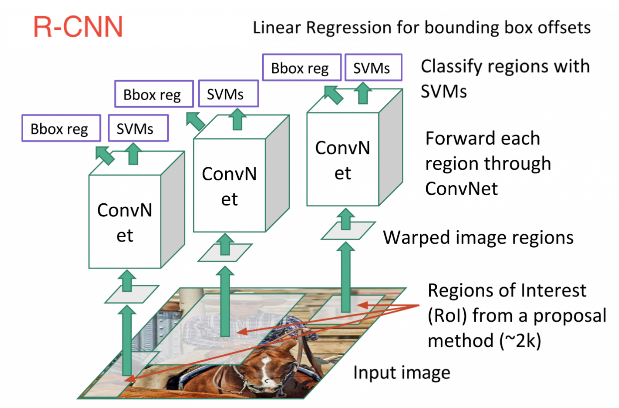
\includegraphics[width=0.7\textwidth]{figures/estado_arte/rcnn.png}
		\caption{Fases de \acrshort{rcnn}}
		\label{fig.rcnn}
		\end{center}
\end{figure}

Por otro lado, Faster \acrshort{rcnn} (Figura~\ref{fig.fast_rcnn}) es una versión más rápida que \acrshort{rcnn}, en la que se modifican algunos aspectos. En este método se incluye la técnica \textit{region proposal}, la cual determina qué regiones de la imagen tienen mayor probabilidad de contener objetos y por tanto cuáles son las regiones que se introducirán en el clasificador. Esto optimiza mucho el trabajo pues evita introducir al clasificador regiones que no sean de interés.


Ignacio Arriola~\cite{tesis_ignacio_arriola} hace también uso de Faster \acrshort{rcnn}. En este trabajo se han entrenado y comparado tres redes Faster \acrshort{rcnn} para la detección de peatones partiendo de diferentes parámetros iniciales. Con ello se pretendía estudiar la transferencia del aprendizaje, experimentando con dos redes pre-entrenadas y una inicializada con parámetros aleatorios.  Las redes pre-entrenadas se trataban de una Faster-\acrshort{rcnn}~\cite{faster_rcnn_ignacio} y una red convolucional Resnet 101 ~\cite{faster_rcnn_regnet_ignacio} como extractor de características. Cada modelo fue entrenado con una base de datos diferente (uno con \textit{\acrfull{coco}}\footnote{http://cocodataset.org/\#home} y otro con KITTI \footnote{http://www.cvlibs.net/datasets/kitti/}).

\begin{figure}[H]
  \begin{center}
    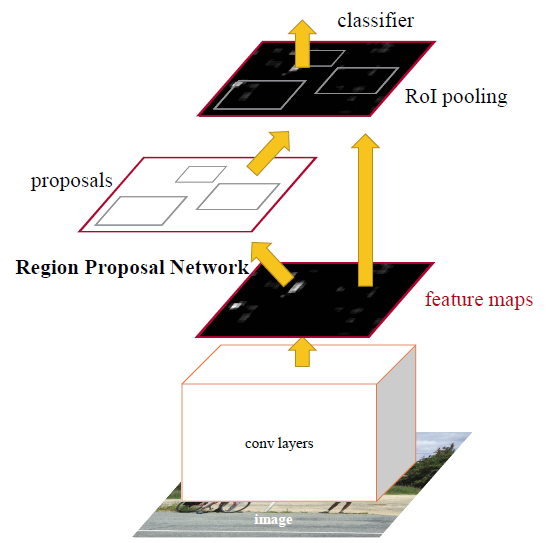
\includegraphics[width=0.5\textwidth]{figures/estado_arte/faster_rcnn.png}
		\caption{Fases de Faster \acrshort{rcnn}}
		\label{fig.fast_rcnn}
		\end{center}
\end{figure}

\subsection*{\acrfull{ssd}}
Otra arquitectura sobresaliente de detección de objetos es el \acrfull{ssd} \cite{ssd}. El principal beneficio de esta arquitectura es el hecho de que integra todos los cálculos necesarios en una sola red neuronal, reduciendo la complejidad en comparación con otras enfoques que requieren propuestas de regiones externas. Esto reduce enormemente el tiempo de cálculo cuando la red tiene que procesar una imagen. La arquitectura puede verse en la Figura \ref{fig:2_arch_ssd_yolo}, y puede dividirse en varias etapas \cite{nacho_tfg}, a saber:
\begin{itemize}
  \item \textbf{\textit{Reshape}}. la primera tarea que debe abordar la red es remodelar la(s) imagen(es) de entrada a un tamaño fijo en el que trabajen el resto de las capas. En el caso de un detector de \acrshort{ssd}, esta forma es n × 300 × 300 × 3 (siendo n el tamaño del lote de entrada, ya que n imágenes pueden ser evaluadas simultáneamente en la red neuronal). Se pueden utilizar otros tamaños de imagen, pero éste ofrece un buen equilibrio entre el rendimiento y la carga de cálculo.
  
  \item \textbf{red base}:  este primer grupo de capas se reutilizan de un modelo típico de clasificación de imágenes, como el VGG-16 \cite{vgg16}. Las primeras capas de esta arquitectura se utilizan en este diseño, truncadas antes de la primera capa de clasificación. De esta manera, la red puede aprovechar los mapas de características de la red de clasificación, para encontrar objetos dentro de la imagen de entrada. Después de la primera parte de la red, se añaden varias capas convolutivas, disminuyendo su tamaño. Esto tiene el objetivo de predecir las detecciones a múltiples escalas. Una cosa que hay que mencionar en este punto es que la red base puede ser una diferente en lugar de la VGG-16, como una \textit{MobileNet} \cite{mobilenet}, que está altamente optimizada para funcionar en dispositivos de gama baja.
  
  \item \textbf{Box predictors}: para cada capa de la red de base, se realiza una convolución de imagen, generando un pequeño conjunto (típicamente 3 o 4) de anclas de tamaño fijo, con diferentes relaciones de aspecto para cada celda de una cuadrícula sobre el mapa de activación (Figura \ref{fig:2_ssd_generated_boxes}). Como estos mapas tienen diferentes tamaños, el sistema es capaz de detectar objetos en diferentes escalas. Las anclas se conviven entonces con pequeños filtros (uno por canal de profundidad), que producen resultados de confianza para cada clase conocida, y compensaciones para el cuadro delimitador generado. Estas puntuaciones se pasan a través de una operación de \textit{softmax}, que los comprime en un vector de probabilidad. Así, para cada objeto detectado (en esa escala), la red calcula la puntuación de cada clase y su posición estimada dentro del mapa de características (por lo tanto, en la imagen también).
  
  \item \textbf{Postprocesamiento}: Dado que pueden producirse varias detecciones en la misma zona para diferentes clases y escalas, se realiza una operación de no máxima supresión [22] a la salida de la red para retener las mejores cajas, bajo un criterio combinado de puntuación de detección y puntuación \textit{IoU} (Intersección sobre Unión), que mide la calidad de superposición entre dos cajas delimitadoras, como puede verse en la figura\ref{fig:2_iou}.
\end{itemize}

\begin{figure}[h]
	\centering
	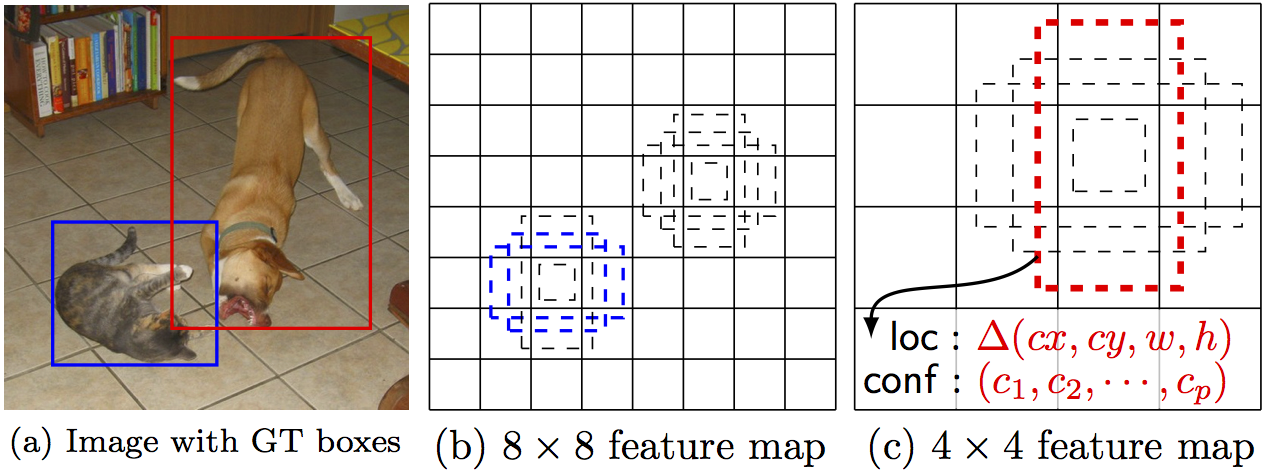
\includegraphics[width=0.7\linewidth]{figures/estado_arte/ssd_generated_boxes.png}
	\caption{Un grupo de cuadrados generados en cada punto de cada mapa de características \cite{ssd}.}
	\label{fig:2_ssd_generated_boxes}
\end{figure}

\begin{figure}[h]
	\centering
	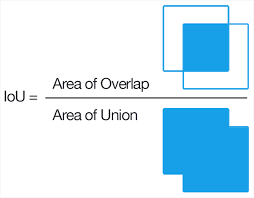
\includegraphics[width=0.4\linewidth]{figures/estado_arte/iou.png}
	\caption{Representación gráfica de una IoU entre dos bounding boxes.}
	\label{fig:2_iou}
\end{figure}

\subsection*{\acrfull{yolo}}
Otro enfoque interesante es el sistema \acrfull{yolo} \cite{yolov1}. Su principal ventaja es su velocidad de inferencia, debido al hecho de que realiza un único análisis de toda la imagen, dividiéndola en una cuadrícula de células. Cada celda predice hasta 5 casillas, que contienen una puntuación de objeto (el IOU predicho de la propuesta con un objeto, independientemente de su clase), las coordenadas de la casilla delimitadora, y una probabilidad para el objeto perteneciente a cada clase. Este diseño funciona más rápido que otros métodos \cite{yolov1}, sin embargo presenta un rendimiento pobre al detectar objetos pequeños. \\

Este diseño fue revisado en \textit{YOLO9000} \cite{yolov2}, introduciendo varias mejoras como la normalización de los lotes a la entrada de las capas convolucionales, o el concepto de cajas de anclaje: las propuestas de cajas siguen un conjunto fijo de relaciones de aspecto, elegidas previamente utilizando la agrupación en un conjunto de entrenamiento. Como puede verse en la figura \ref{fig:2_yolov2_anchor_clustering}, la limitación de las formas de la propuesta a 5 tamaños fijos mejora el rendimiento, manteniendo al mismo tiempo un alto \textit{IuO}. Una inspección visual muestra que las anclas seleccionadas parecen tener una forma razonable para la mayoría de los objetos que la red pretende detectar. Además, el número de capas profundas fue aumentó de 26 capas a 30, y se realiza un modelado semántico en las etiquetas a través de diferentes conjuntos de datos, lo que permite a la red capacitarse en diferentes conjuntos de datos bajo una estructura semántica llamada \textit{WordTree} (Figura \ref{fig:2_yolov2_wordtree}).
\begin{figure}[H]
	\centering
	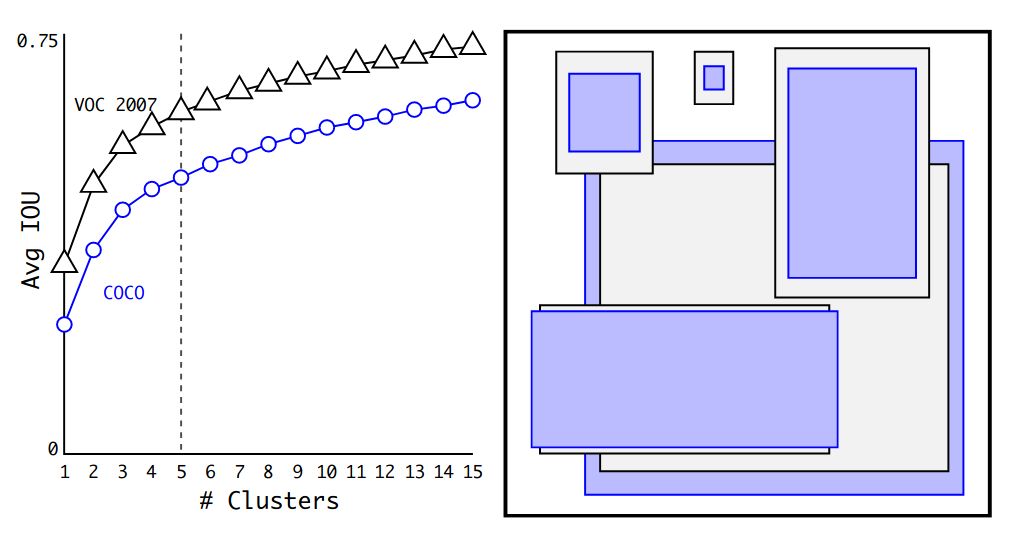
\includegraphics[width=0.6\linewidth]{figures/estado_arte/yolov2_anchor_clustering.png}
	\caption{El resultado del ancla k significa agrupación en VOC y COCO para YOLO9000. Usar tamaños de ancla de $k=5$ en la derecha produce un buen equilibrio entre la simplicidad y la mejora en el IuO obtenido con respecto a usar clusters de $k-1$ (source: \cite{yolov2}).}
	\label{fig:2_yolov2_anchor_clustering}
\end{figure}

\begin{figure}[h]
	\centering
	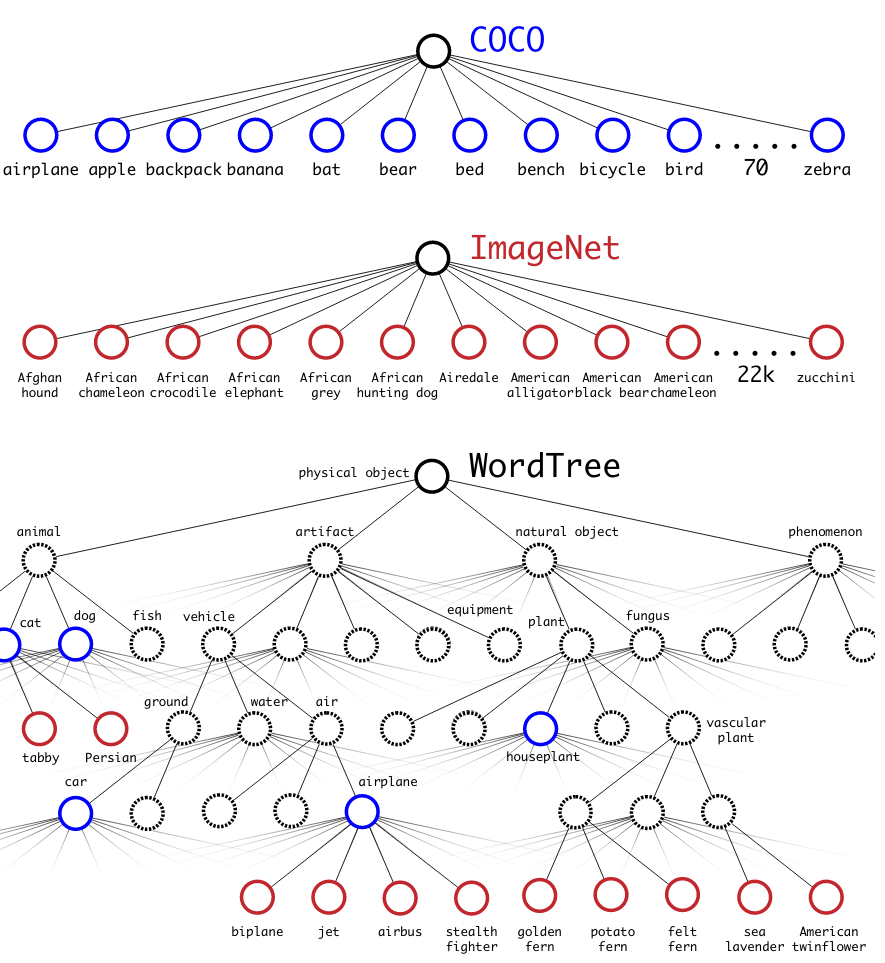
\includegraphics[width=0.6\linewidth]{figures/estado_arte/yolov2_wordtree.png}
	\caption{Comparación entre estructuras de etiquetado simples (arriba) y una agrupación semántica de WordTree bajo categorías (abajo). Esto permite seguir un proceso de formación de datos agnóstico, ya que las etiquetas pueden combinarse utilizando WordTree. Imagen de \cite{yolov2}.}
	\label{fig:2_yolov2_wordtree}
\end{figure}
La última mejora de \acrshort{yolo}, \textit{YOLOv3} \cite{yolov3}, se basa en redes residuales  \cite{resnets}, que abordan el problema de la desaparición de los gradientes cuando las redes se hacen más profundas.
El apilamiento de varias capas resulta en gradientes que disminuyen su valor hasta un punto que la precisión aritmética de la máquina no es capaz de manejar. Los gradientes se cancelan, dificultando el proceso de formación, ya que los parámetros de las primeras capas tardan un tiempo sustancialmente mayor en converger. Las redes residuales añadidas en esta revisión del diseño añaden conexiones de atajo a través de las capas, centrando los gradientes de retropropagación en las diferencias entre la entrada y la salida de la capa. Como dice esta referencia \cite{yolov3}, la combinación de estas capas residuales y las convolucionales permite entrenar arquitecturas mucho más profundas (53 capas convolucionales), capaces de producir una mayor generalización. Al igual que en los detectores de \acrshort{ssd}, la arquitectura \acrshort{yolo} realiza detecciones a múltiples escalas, utilizando 3 escalas para dividir los mapas de características en cuadrículas de células. En el conjunto de datos \acrshort{coco} se realiza una agrupación similar a la de la figura 2.10, seleccionando 9 tamaños de ancla en lugar de 5, y agrupándolos en 3 escalas. Ahora, en cada una de las celdas, caben 9 cajas delimitadoras de anclas (3 formas de anclas × 3 escalas). Esto tiene como objetivo mejorar el pobre rendimiento de la versión anterior cuando se trata de objetos pequeños, así como producir una mejor generalización: en el \textit{R-CNN} [16] y en el \acrshort{ssd} [19] las formas de anclaje se seleccionan a mano. Estos cambios, con un ajuste en la función de error, conforman las mejoras de \textit{YOLOv3} sobre las versiones anteriores.

Para (ancla, celda, escala) combinación, \textit{YOLOv3} predice:
\begin{itemize}
  \item Las coordenadas del objeto dentro del ancla. Los detalles se pueden visualizar en la figura 2.12.
  \item \textit{Puntuación de objetividad}, que se calcula mediante una regresión logística a fin de maximizar la probabilidad de superposición con un cuadro delimitador de la verdad del terreno con respecto a la de cualquier otra ancla anterior.
  \item 80 puntos, ya que la implementación original está entrenada en el conjunto de datos del COCO, que contiene 80 clases. Estas clases pueden estar superpuestas (por ejemplo, "woman" y "person"). Por lo tanto, estas puntuaciones son calculadas por clasificadores logísticos independientes y no se pasan por una operación de softmax.
\end{itemize}

\begin{figure}[H]
	\centering
	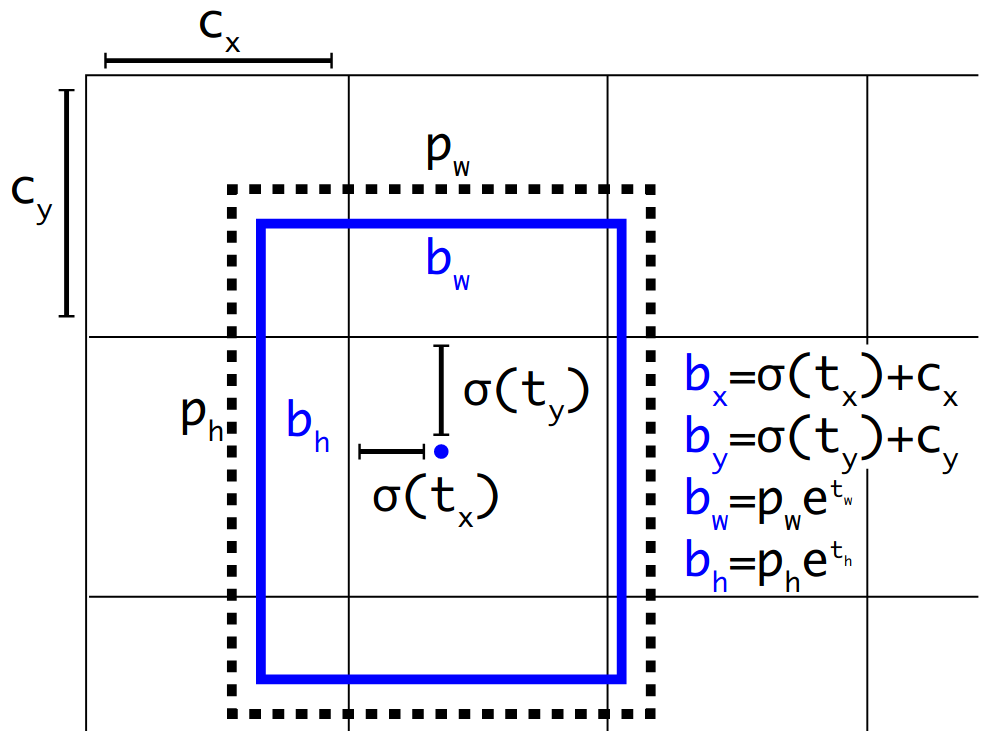
\includegraphics[width=0.5\linewidth]{figures/estado_arte/yolo_outputs.png}
	\caption{Salida en \acrshort{yolo} para cada ancla y célula. La línea discontinua representa el ancla anterior, mientras que la línea azul representa la detección que corrige esa ancla.}
	\label{fig:2_yolo_output}
\end{figure}

La arquitectura de una red de detección basada en \acrshort{yolo} puede compararse con la de una basada en \acrshort{ssd} en la figura 2.13. Esto permite ver la diferencia fundamental en la etapa de extracción de características de cada enfoque.

\begin{figure}[h]
	\centering
	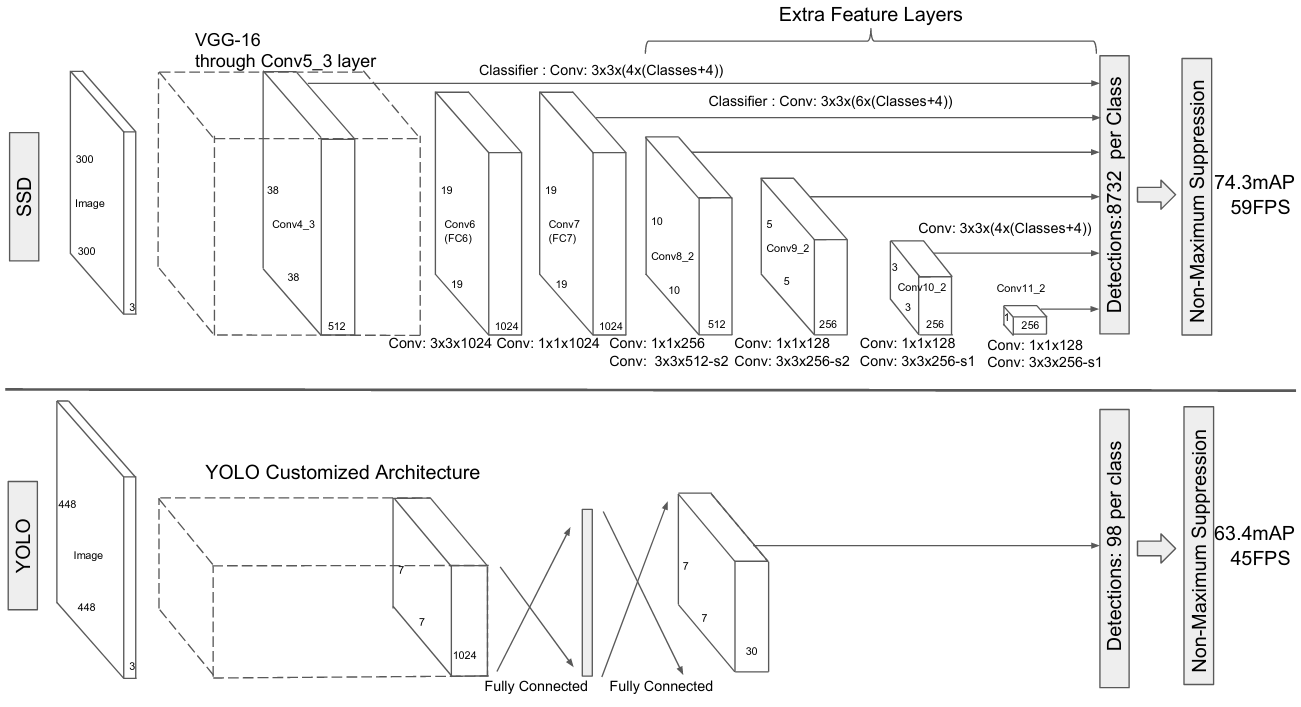
\includegraphics[width=0.8\linewidth]{figures/estado_arte/arch_ssd_yolo.png}
	\caption{Arquitectura general de una red \acrshort{ssd} (arriba) y una \acrshort{yolo} (abajo). Imagen de \cite{ssd}.}
	\label{fig:2_arch_ssd_yolo}
\end{figure}
\section{Bases de datos de detección visual de objetos}
La detección visual de personas pretenden encontrar una persona en una imagen o en un vídeo. Dado que queremos encontrar la persona en cuestión bajo diferentes circunstancias, es decir, en distintos entornos y diferentes iluminaciones, necesitaremos típicamente entrenar el modelo con un conjunto de imágenes representativo. Por este motivo, a lo largo de los últimos años han surgido en la comunidad internacional diferentes \textit{datasets} con el fin de solucionar este problema.

\subsection{\acrfull{coco}}
El \textit{dataset} de \acrfull{coco}\footnote{\url{https://cocodataset.org}}\cite{cocodataset} es uno de los conjuntos de imágenes mas usados para entrenar redes para detección de objetos. Esto se debe a que contiene mas de 200.000 imágenes etiquetadas (figura \ref{fig.coco}) con en torno a 80 clases de objetos diferentes. Además no solo se usa para detección, también para segmentación, clasificación y otros usos.

\begin{figure}[H]
  \begin{center}
    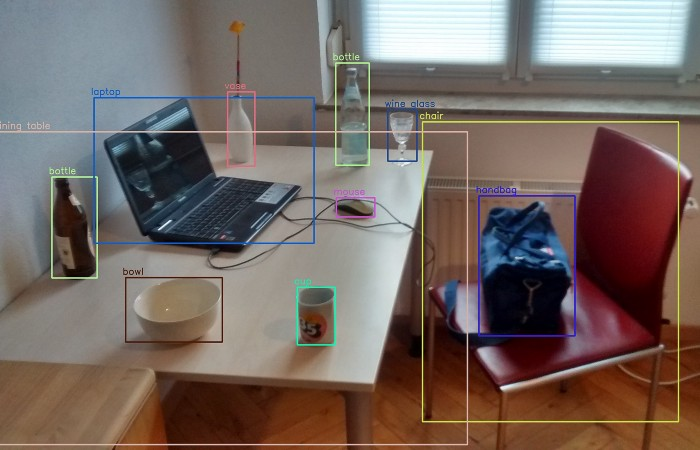
\includegraphics[width=0.8\textwidth]{figures/estado_arte/coco.jpeg}
		\caption{ejemplo de \textit{\acrshort{coco}}}
		\label{fig.coco}
		\end{center}
\end{figure}

\subsection{Open Images}
\textit{Open Images}\footnote{\url{https://storage.googleapis.com/openimages/web/index.html}}~\cite{OpenImages} es un conjunto de datos de aproximadamente 9 millones de imágenes anotadas (figura \ref{fig.oi}) con etiquetas de nivel de imagen, cajas delimitadoras de objetos, máscaras de segmentación de objetos, relaciones visuales y narraciones localizadas. Las cajas han sido dibujadas en gran parte manualmente por anotadores profesionales para garantizar la precisión y la coherencia. Las imágenes son muy diversas y a menudo contienen escenas complejas con varios objeto. 

También ofrece anotaciones de relaciones visuales, indicando pares de objetos en relaciones particulares (por ejemplo, "mujer tocando la guitarra"), propiedades de los objetos (por ejemplo, "la mesa es de madera") y acciones humanas (por ejemplo, "la mujer está saltando").

\begin{figure}[H]
  \begin{center}
    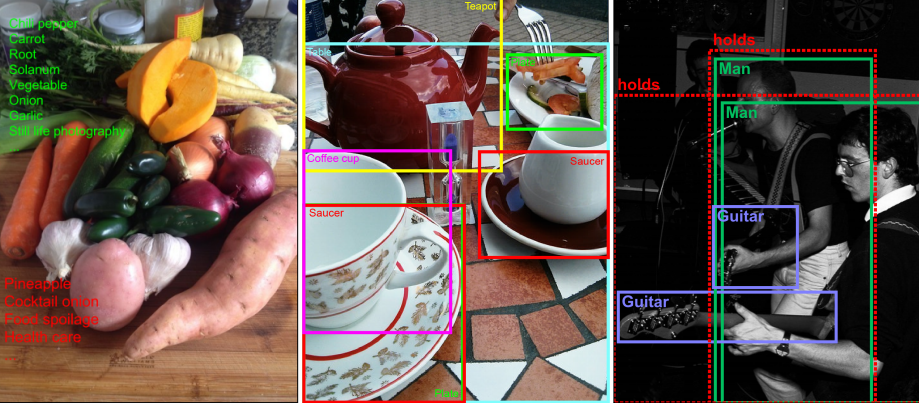
\includegraphics[width=0.8\textwidth]{figures/estado_arte/openImages.png}
		\caption{ejemplo de \textit{Open Images}}
		\label{fig.oi}
		\end{center}
\end{figure}

\subsection{\acrfull{voc} 2012}

Este conjunto de datos contiene los datos del \textit{\acrfull{voc}} 2012\footnote{\url{http://host.robots.ox.ac.uk/pascal/VOC/voc2012/}}~\cite{pascal-voc-2012}, también conocido como \textit{VOC2012}, correspondiente a las competiciones de Clasificación y Detección. Un total de 11540 imágenes están incluidas en este conjunto de datos, donde cada imagen contiene un conjunto de objetos, de 20 clases diferentes, haciendo un total de 27450 objetos anotados.

\subsection{ImageNet}
El proyecto ImageNet\footnote{\url{http://image-net.org/index}} es una gran base de datos visual diseñada para su uso en la investigación de software de reconocimiento visual de objetos. Contine más de 14 millones de imágenes anotadas a mano para indicar qué objetos se han fotografiado y en al menos un millón de las imágenes también se proporcionan recuadros delimitadores. Además contiene más de 20.000 categorías.